\subsection{Trees}

\subsubsection{Definitions and characteristics}

Before introducing what a tree is, it is necessary to understand what a subgraph is. Mathematically speaking, $G'= \left(N', E'\right)$ is a \definitionWithSpecificIndex{subgraph}{Subgraph} of $G = \left(N,E\right)$ if $N' \subseteq N$ and $E' \subseteq E$.

\highspace
A \definitionWithSpecificIndex{tree of the graph $G$}{Tree of a graph} is a connected and acyclic subgraph of $G$ and it is represented as $G_{T} = \left(N', T\right)$. If the tree contains exactly every node in the graph $G$, it is called the \definitionWithSpecificIndex{spanning tree}{Spanning tree} of $G$ and is represented as $G_{T} = \left(N', T\right)$. Finally, we call the \textbf{nodes of degree 1} in a tree as \definitionWithSpecificIndex{leaves}{Leaves of a tree}.

\begin{examplebox}[: subgraph, tree and spanning tree]
    Given a graph $G$:
    \begin{center}
        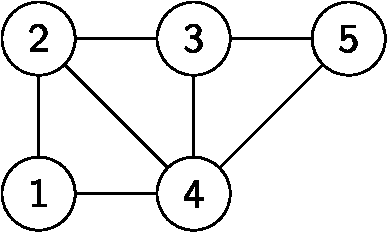
\includegraphics[width=.3\textwidth]{img/trees-1.pdf}
    \end{center}

    \begin{itemize}
        \item The following figure is a \textbf{subgraph} of $G$, but \underline{not} a tree, because there is a cycle $\left(1,2,4\right)$.
        \begin{center}
            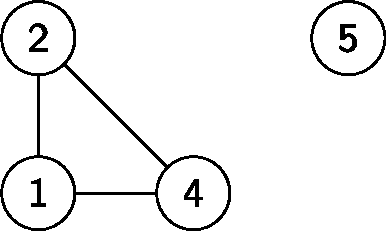
\includegraphics[width=.3\textwidth]{img/trees-2.pdf}
        \end{center}

        \item The following figure is a \textbf{subgraph} of $G$, and it is a \textbf{tree} because there are no cycles and the graph is connected.
        \begin{center}
            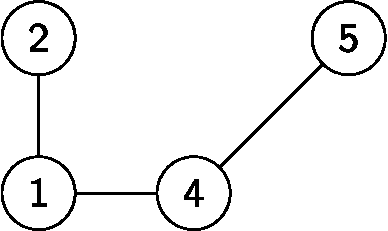
\includegraphics[width=.3\textwidth]{img/trees-3.pdf}
        \end{center}
        
        \item The following figure is a \textbf{spanning tree} of $G$ because it contains all the nodes in $G$, and it is a tree because it is connected and acyclic.
        \begin{center}
            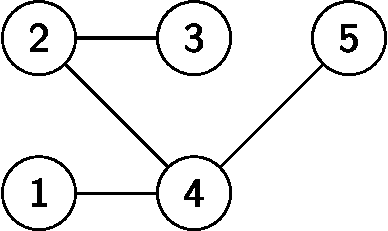
\includegraphics[width=.3\textwidth]{img/trees-4.pdf}
        \end{center}
    \end{itemize}
\end{examplebox}

\newpage

\subsubsection{Properties}

\begin{enumerate}
    \item \textbf{Every tree with $n$ nodes has $n-1$ edges}.
    \begin{proof}[Inductive proof]
        Base case: the claim holds for $n=1$ (tree with $1$ node and $0$ edges).

        Inductive step: show that, if this is true for trees with $n$ nodes, then it is also true for those with $n+1$ nodes.

        Let $T_{1}$ be a tree with $n+1$ nodes and recall that any tree with $n \ge 2$ nodes has at least $2$ leaves (two nodes of degree 1, the number of incident edges). By deleting one leaf and its incident edge, we obtain a tree $T_{2}$ with $n$ nodes. By induction hypothesis, $T_{2}$ has $n-1$ edges. Therefore, the tree $T_{1}$ has $n-1+1 = n$ edges.
    \end{proof}

    \item \textbf{Every pair of nodes in a tree is connected by a unique path}. The proof is not necessary, because otherwise there would be a cycle (and this is against the definition of a tree).

    \item \textbf{By adding a new edge to a tree, we can create a unique cycle}.

    \item Let $G_{T} = \left(N,T\right)$ be a spanning tree of $G = \left(N,E\right)$. Consider an edge $e \notin T$ and the unique cycle $C$ of $T \cup \left\{e\right\}$ (as in property 3). For each edge $f \in C \setminus \left\{e\right\}$, the subgraph $T \cup \left\{e\right\} \setminus \left\{f\right\}$ is also a spanning tree of $G$.
    \begin{figure}[!htp]
        \centering
        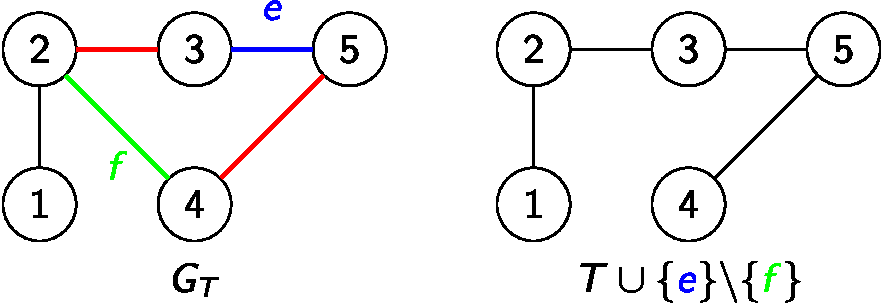
\includegraphics[width=.5\textwidth]{img/trees-5.pdf}
    \end{figure}

    \item Let $F$ be a partial tree (spanning nodes in $S \subseteq N$) contained in an optimal tree of $G$. Consider $e = \left\{u,v\right\} in \delta\left(S\right)$ of minimum cost, then there exists a minimum cost spanning tree of $G$ containing $e$ (is better explained in the \ref{paragraph: Prim's algorithm} paragraph, page \pageref{paragraph: Prim's algorithm}).

    \begin{proof}
        By contradiction, assume $T^{*} \subseteq E$ is a minimum cost spanning tree with $F \subseteq T^{*}$ and $e \notin T^{*}$. Adding edge $e$ to $T^{*}$ creates the cycle $C$. Let $f \in \delta\left(S\right) \cap C$.
        \begin{itemize}
            \item If $c_{e} = c_{f}$, then $T^{*} \cup \left\{e\right\} \setminus \left\{f\right\}$ is (also) optimal since it has same cost of $T^{*}$.
            
            \item If $c_{e} < c_{f}$, then $c\left(T^{*} \cup \left\{e\right\} \setminus \left\{f\right\}\right) < c\left(T^{*}\right)$, hence $T^{*}$ is not optimal.
        \end{itemize}
        \begin{figure}[!htp]
            \centering
            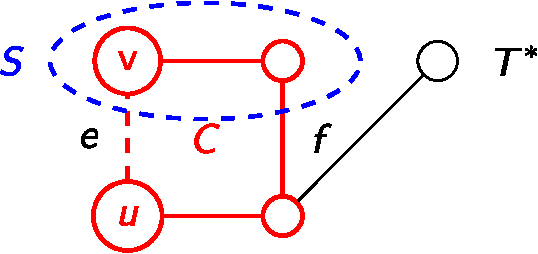
\includegraphics[width=.4\textwidth]{img/trees-9.pdf}
        \end{figure}
    \end{proof}
\end{enumerate}

\newpage

\subsubsection{Optimal cost spanning trees}

Spanning trees are very common because they are used in a wide range of applications such as network design, IP network protocols, enterprise storage, etc.

\begin{examplebox}[: introduction to finding the best and optimal cost solution]
    Design a communication network so as to connect $n$ cities at \textbf{minimum total cost}.

    The model is made up as follows:
    \begin{itemize}
        \item Graph $G = \left(N,E\right)$ with $n = \left| N \right|$, $m = \left| E \right|$
        \item Cost function $c: E \rightarrow c_{e} \in \mathbb{R}$, with $e = \left\{u,v\right\} \in E$.
    \end{itemize}
    \begin{center}
        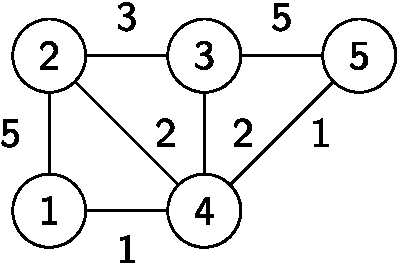
\includegraphics[width=.3\textwidth]{img/trees-6.pdf}
    \end{center}

    The required properties are:
    \begin{itemize}
        \item Each pair of cities must communicate, then the connected subgraph containing all the nodes.
        \item The minimum total cost, then the subgraph must have no cycles.
    \end{itemize}

    We give two solutions, where the second is better because it is more feasible and optimal:
    \begin{enumerate}
        \item $c\left(T_{1}\right) = 15$
        \begin{center}
            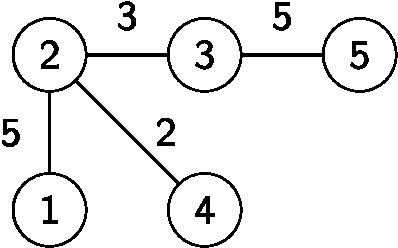
\includegraphics[width=.3\textwidth]{img/trees-7.pdf}
        \end{center}

        \item $c\left(T_{2}\right) = 6$
        \begin{center}
            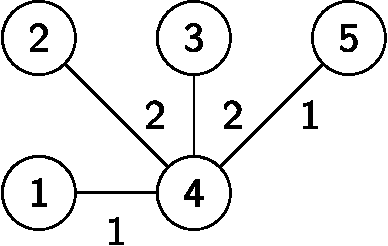
\includegraphics[width=.3\textwidth]{img/trees-8.pdf}
        \end{center}
    \end{enumerate}
\end{examplebox}

\newpage

\noindent
In general, we can formalize the \definitionWithSpecificIndex{optimal cost}{Optimal Cost} as follows. Given an undirected graph $G = \left(N,E\right)$ and a cost function, \textbf{find a spanning tree} $G_{T} = \left(N, T\right)$ \textbf{of minimum total cost}:
\begin{equation}
    \underset{T \in X}{\min} \displaystyle\sum_{e \in T} c_{e} \hspace{2em} \text{where } X \text{ is the set of all spanning trees of } G
\end{equation}

\highspace
Doesn't exists only one spanning tree, they are multiples. But the number of spanning trees available in a complete graph is defined by a theorem.
\begin{theorem}[Cayley, 1889]
    A complete graph with $n$ nodes ($n \ge 1$) has $n^{n-2}$ spanning trees.
\end{theorem}

\noindent
In general, the problem of finding a spanning tree with minimum total cost is also called \definitionWithSpecificIndex{minimum spanning tree (MST) problem}{minimum spanning tree (MST) problem}. It plays an important role in many networking applications, such as routing and networking.\cite{10.1007/978-3-642-38853-8_14}

\newpage

\paragraph{Prim's algorithm}\label{paragraph: Prim's algorithm}

\begin{definitionbox}[: Prim's]
    \definition{Prim's algorithm} is a \textbf{greedy algorithm that finds a minimum spanning tree for a weighted undirected graph}. This means it \textbf{finds a subset of the edges that forms a tree that includes every vertex, where the total weight of all the edges in the tree is minimized}. The algorithm operates by building this tree one vertex at a time, from an arbitrary starting vertex, at each step adding the cheapest possible connection from the tree to another vertex. Finally, \textbf{Prim's algorithm is exact} (it provides an optimal solution for every instance).
\end{definitionbox}

\highspace
A \definitionWithSpecificIndex{greedy algorithm}{Greedy algorithm} constructs a \textbf{feasible solution iteratively by making a \dquotes{locally optimal} choice at each step, without reconsidering previous choices}. In Prim's algorithm, at each step a minimum-cost edge is selected from those in the cut $\delta\left(S\right)$ induced by the current set of nodes $S$. Unfortunately, for most discrete optimization problems greedy-type algorithms yield a feasible solution with no guarantee of optimality.

\highspace
According to the definition of a greedy algorithm, the main idea of Prim is to build a spanning tree iteratively. It \textbf{starts with an initial tree} $\left(S,T\right)$ with $S = \left\{u\right\}$ ($u \in N$, so it can be any node in the set $N$) and $T = \emptyset$. At \textbf{each step}, \textbf{add} to the current sub-tree $\left(S,T\right)$ \textbf{a minimum cost edge} among those that connect a node in $S$ to a node in $N \setminus S$.

\begin{examplebox}[: Prim's algorithm]
    Suppose we have the following graph:
    \begin{center}
        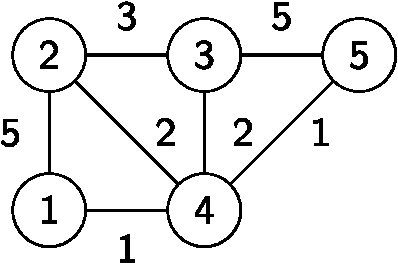
\includegraphics[width=.3\textwidth]{img/prims-alg-1.pdf}
    \end{center}

    \begin{enumerate}
        \item We start from an arbitrarily node $u$ that it is in the set $N$, for example $3$:
        \begin{center}
            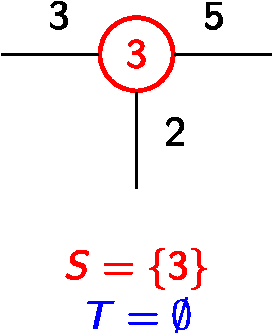
\includegraphics[width=.2\textwidth]{img/prims-alg-2.pdf}
        \end{center}

        \item As we said, at each step we add to the current subtree $\left(S, T\right)$ a minimum cost edge among those that connect a node in $S$ to a node in $N \setminus S$. So at this step we choose \emph{node 4} because the edge starting from \emph{node 3} is the less weighted edge.
        \begin{center}
            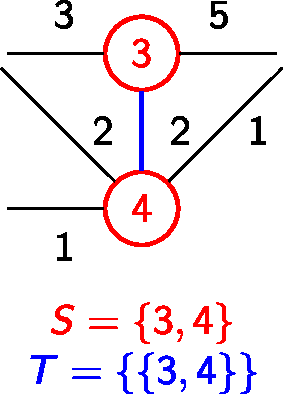
\includegraphics[width=.2\textwidth]{img/prims-alg-3.pdf}
        \end{center}

        \item At this point we continue with the same logic. The edge, starting from \emph{node 4}, with less weighted edge is \emph{node 1}. Note that at parity of the weighted edge, it doesn't matter which one we choose. Maybe the decision will lead to a different subgraph, but Prim's algorithm is greedy by definition, then it doesn't think about these problems; it assumes that it is a locally optimal choice.
        \begin{center}
            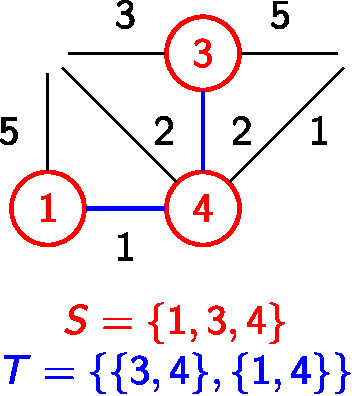
\includegraphics[width=.25\textwidth]{img/prims-alg-4.pdf}
        \end{center}

        \item Since we are lucky, the previous doubt is useless (with parity of weighted vertices, which should we choose?). Because \emph{node 1} exposes an edge with a weight of 5, but \emph{node 4} has a weighted edge of only 1, the choice is clear.
        \begin{center}
            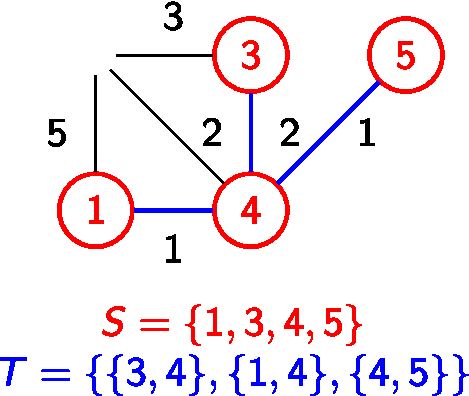
\includegraphics[width=.3\textwidth]{img/prims-alg-5.pdf}
        \end{center}

        \item Finally, we choose the edge with a weight of 2 (to the \emph{node 2}) because is the lowest. At this step, the algorithm is finished because there are no more vertices ($S = N$). The cost function returns the value $6$ (sum of each weighted edge selected).
        \begin{center}
            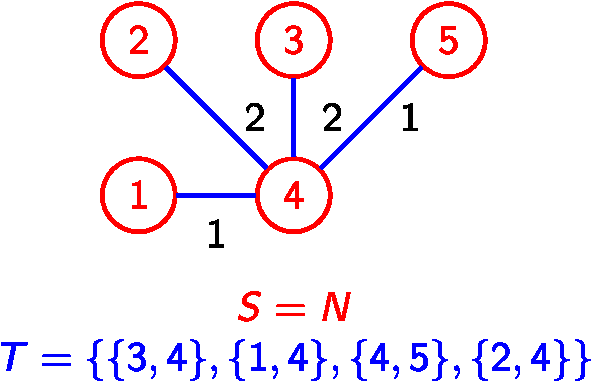
\includegraphics[width=.4\textwidth]{img/prims-alg-6.pdf}
        \end{center}
    \end{enumerate}
\end{examplebox}

\noindent
From the previous example it should be clear that at each step the Prim's algorithm creates the need to solve a minimum search problem.

\highspace
The Prim's algorithm take:
\begin{itemize}
    \item Input: a connected graph $G = \left(N,E\right)$ with edge costs.
    \item Output: a subset $T \subseteq N$ of edges of $G$ such that $G_{T} = \left(N,T\right)$ is a minimum cost spanning tree of $G$.
\end{itemize}

\begin{lstlisting}[language=pseudo-code, caption={Minimum spanning tree (MST) problem: Prim's $O\left(nm\right)$}]
S $\leftarrow$ $\{$u$\}$; $\label{prims: s-definition}$
T $\leftarrow$ $\emptyset$; $\label{prims: t-definition}$
while $\left|T\right| < n-1$ do: $\label{prims: while cycle}$
    $\left\{u\right\} \leftarrow$ edge in $\delta(S)$ of minimum cost; // with $u \in S$ and $v \in N \setminus S$ $\label{prims: search minimum}$
    $S \leftarrow S \cup \left\{v\right\}$; $\label{prims: add destination vertex}$
    $T \leftarrow T \cup \left\{\left\{u,v\right\}\right\}$ $\label{prims: add tuple source destination}$
\end{lstlisting}
\begin{itemize}
    \item[Rows \ref{prims: s-definition}-\ref{prims: t-definition}.] Declare the general sets $S$ and $T$. The first is filled with the starting node $u$ and the second is empty, because the core of the algorithm has not yet started.

    \item[Row \ref{prims: while cycle}.] Continue building the spanning tree until the length of the set of transitions $T$ is not equal to the number of nodes minus one.

    \item[Row \ref{prims: search minimum}.] Find the edge with the lowest weight from the set $\delta\left(S\right)$. Then choose one of the edges with the lowest weight and the corresponding target node. Obviously the target node $v$ cannot be already evaluated ($v \in N \setminus S$) and the source node $u$ must be in the set of nodes already evaluated ($u \in S$).
    
    \item[Rows \ref{prims: add destination vertex}-\ref{prims: add tuple source destination}.] Therefore, the most complex part of the algorithm (minimum search) is to store the target vertex with the lowest edge weight and add the tuple (source node, target node) to the set $T$.
\end{itemize}
The complexity of the algorithm is pretty much guessed. Or in the better case neither worst case, we need to evaluate each node. Then the main difference is made by the weighted edge search. If each edge has to be analyzed at each iteration, the \textbf{complexity} order is given by $O\left(nm\right)$.

\newpage

\paragraph{Implementation of Prim's algorithm in $O\left(n^{2}\right)$}

Prim's algorithm is based on graph traversals (visiting every vertex in the graph), which are inherently difficult to parallelize. It also has an irregular memory access pattern. In CPUs, this limits the use of the cache and leads to an overall performance penalty. The prim's algorithm is highly dependent on the organization of memory storage and memory access patterns.\cite{10.1007/978-3-642-38853-8_14}

\highspace
The following data structure we propose guarantees a complexity of $O\left(n^{2}\right)$.
\begin{itemize}
    \item $k$ is the number of edges selected so far;

    \item $S$ is the subset $S \subseteq N$ of nodes incident to the selected edges (same as explained in the \ref{paragraph: Prim's algorithm} section, page \pageref{paragraph: Prim's algorithm});
    
    \item $T$ is the subset $T \subseteq E$ of selected edges (same as explained in the \ref{paragraph: Prim's algorithm} section, page \pageref{paragraph: Prim's algorithm});
    
    \item $C_{j}$ is a vector which has a value equal to:
    \begin{equation*}
        C_{j} = \begin{cases}
            \min\left\{c_{ij} \: : \: i \in S\right\} & j \notin S \\
            \infty & \text{otherwise}
        \end{cases}
    \end{equation*}
    At the beginning of the algorithm it is clearly composed of infinite values if the edge $i$ to $j$ doesn't exist, otherwise the weight of the edge. In the core of the algorithm, each position is updated with the minimum weighted edge value.
    
    \item $\text{closest}_{j}$ is a vector which has a value equal to:
    \begin{equation*}
        \text{closest}_{j} = \begin{cases}
            \mathrm{argmin}\left\{c_{ij} \: : \: i \in S\right\} & j \notin S \\
            \text{predecessor of }j\text{ in the minimum spanning tree} & j \in S
        \end{cases}
    \end{equation*}
    The node closest to the edge has less weight, otherwise if we look at the node $j$ in the set $S$, the predecessor of that node in the minimum spanning tree. A trivial example:
    \begin{figure}[!htp]
        \centering
        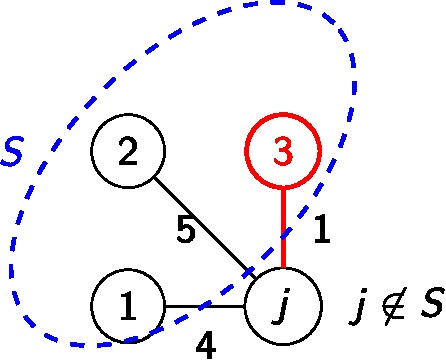
\includegraphics[width=.3\textwidth]{img/prims-alg-7.pdf}
    \end{figure}
    
    With $\mathrm{closest}_{j} = 3$ and $c_{\mathrm{closest}_{j}},j = 1$.
\end{itemize}
Let's take an example to clear up any doubts.

\begin{examplebox}[: Prim's algorithm $O\left(n^{2}\right)$]
    Suppose we have the following graph:
    \begin{center}
        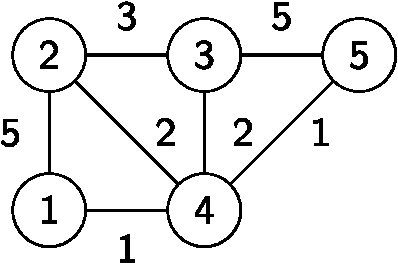
\includegraphics[width=.3\textwidth]{img/prims-alg-1.pdf}
    \end{center}

    \begin{enumerate}
        \item At the beginning we choose an arbitrary node $u$ that is in the set $N$, for example $3$. We set the set of transitions $T$ to the empty set, the set of evaluated nodes $S$ to the selected node $u$, in our case the value 3, and finally the two vectors. The vector $C_{j}$ is filled of infinite values if the edge $u$ to $j$ doesn't exist, otherwise the weight of the edge, and the vector $\text{closest}_{j}$ is filled with the selected starting node, in our case 3.
        \begin{itemize}
            \item $T = \emptyset$
            \item $S = \left\{u\right\} = \left\{3\right\}$
            \item $C_{j} = \left[+\infty, 3, -, 2, 5\right]$
            \item $\text{closest}_{j} = \left[3, 3, -, 3, 3\right]$
        \end{itemize}
        Some observations:
        \begin{itemize}
            \item The symbol $-$ is the \href{https://en.wikipedia.org/wiki/Don%27t-care_term}{don't care term used in digital logic}.
            \item The position of each value respects the j-index. For example, the node 3 in the vectors $C_{j}$ and $\text{closest}_{j}$ is placed at position number 3. The value is don't care ($-$) because it is the starting point. The other values depend on the graph. Node 1 has no direct edge to node 3, so it has an infty value; node 2 has a direct edge with weight 3; node 3 doesn't care because it's the starting point; and so on.
        \end{itemize}
        \begin{center}
            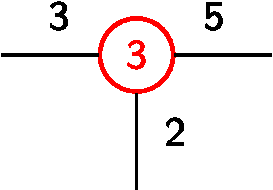
\includegraphics[width=.2\textwidth]{img/prims-alg-2-imp.pdf}
        \end{center}

        \item The minimum value in $C_{j}$ is 2 and since it is in the 4th position, node 4 is selected.
        \begin{itemize}
            \item $T = \left\{\left\{3,4\right\}\right\}$
            \item $S = \left\{3, 4\right\}$
            \item $C_{j} = \left[\mathbf{1}, \mathbf{2}, -, 2, \mathbf{1}\right]$
            \item $\text{closest}_{j} = \left[\mathbf{4}, \mathbf{4}, -, 3, \mathbf{4}\right]$
        \end{itemize}
        The values updated are the first, second and fifth positions, as nodes three and four are in the $S$ set.
        \begin{center}
            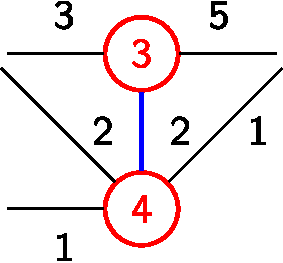
\includegraphics[width=.2\textwidth]{img/prims-alg-3-imp.pdf}
        \end{center}

        \item The minimum value in $C_{j}$ is the first position. But the fifth position is also the minimum. We choose the first value because the vector is analyzed sequentially (first to last).
        \begin{itemize}
            \item $T = \left\{\left\{3,4\right\}, \left\{1,4\right\}\right\}$
            \item $S = \left\{1, 3, 4\right\}$
            \item $C_{j} = \left[1, \mathbf{2}, -, 2, \mathbf{1}\right]$
            \item $\text{closest}_{j} = \left[4, \mathbf{4}, -, 3, \mathbf{4}\right]$
        \end{itemize}
        \begin{center}
            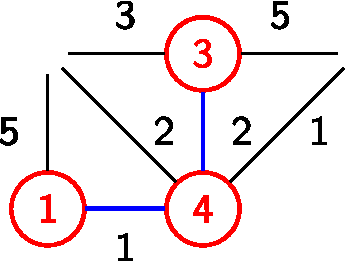
\includegraphics[width=.25\textwidth]{img/prims-alg-4-imp.pdf}
        \end{center}

        \item The minimum value in $C_{j}$ is quite trivial, between 2 and 1. We choose the value 1 and the node $4$ is the closest.
        \begin{itemize}
            \item $T = \left\{\left\{3,4\right\}, \left\{1,4\right\}, \left\{4,5\right\}\right\}$
            \item $S = \left\{1, 3, 4, 5\right\}$
            \item $C_{j} = \left[1, \mathbf{2}, -, 2, 1\right]$
            \item $\text{closest}_{j} = \left[4, \mathbf{4}, -, 3, 4\right]$
        \end{itemize}
        \begin{center}
            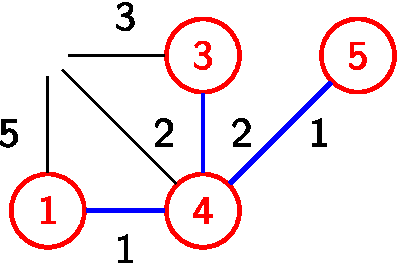
\includegraphics[width=.3\textwidth]{img/prims-alg-5-imp.pdf}
        \end{center}

        \item Finally, node 2 with edge weight 2 is selected.
        \begin{itemize}
            \item $T = \left\{\left\{3,4\right\}, \left\{1,4\right\}, \left\{4,5\right\}, \left\{2,4\right\}\right\}$
            \item $S = \left\{1, 2, 3, 4, 5\right\} = N$
            \item $C_{j} = \left[1, 2, -, 2, 1\right]$
            \item $\text{closest}_{j} = \left[4, 4, -, 3, 4\right]$
        \end{itemize}
        \begin{center}
            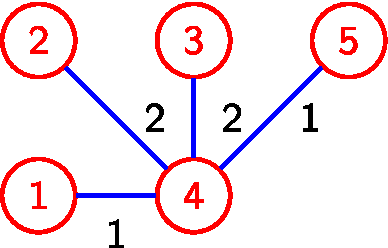
\includegraphics[width=.3\textwidth]{img/prims-alg-6-imp.pdf}
        \end{center}
    \end{enumerate}
\end{examplebox}

\noindent
\begin{flushleft}
    \textcolor{Green3}{\faIcon{question-circle} \textbf{Ok, but how do we get the spanning tree from the nearest vector?}}
\end{flushleft}
The minimum spanning tree found by Prim's algorithm consists of the $n-1$ edges:
\begin{equation*}
    \left\{\text{closest}_{j}, j\right\} \hspace{2em} \text{with } j = 1,2,\dots,n
\end{equation*}
For example, from the previous example, let the \emph{closest} vector:
\begin{equation*}
    \text{closest}_{j} = \left[4,4,-,3,4\right]
\end{equation*}
A minimum cost spanning tree consists of the edges:
\begin{equation*}
    \left\{4,1\right\}, \left\{4,2\right\}, \cancel{\left\{-,-\right\}}, \left\{3,4\right\}, \left\{4,4\right\}
\end{equation*}
\begin{lstlisting}[language=pseudo-code, caption={Minimum spanning tree (MST) problem: Prim's $O\left(n^{2}\right)$}]
S $\leftarrow$ $\{$u$\}$; $\label{prims-imp: s-definition}$
T $\leftarrow$ $\emptyset$; $\label{prims-imp: t-definition}$
for $j \in N \setminus S$ do: $\label{prims-imp: for j in N setminus S}$
    $C_{j} \leftarrow c_{uj}$; // or $+\infty$ if $\left\{u,j\right\} \notin E$
    $\text{closest}_{j} \leftarrow u$; $\label{prims-imp: end for}$
for $k = 1, \dots, n-1$ do: $\label{prims-imp: for k from 1 to n-1}$
    // select min edge in $\delta(S)$
    min $\leftarrow +\infty$; $\label{prims-imp: start select minimum edge}$
    for $j = 1, \dots, n$ do: $\label{prims-imp: third for}$
        if $j \notin S$ and $C_{j} <$ min:
            min $\leftarrow C_{j}$;
            v $\leftarrow$ j; $\label{prims-imp: end select minimum edge}$
    // extend S and T
    S $\leftarrow$ S $\cup \left\{v\right\}$; $\label{prims-imp: start extend S and T}$
    T $\leftarrow$ T $\cup \left\{\left\{\text{closest}_{v}, v\right\}\right\}$; $\label{prims-imp: end extend S and T}$
    // update $C_{j}$ and $\text{closest}_{j}$, $\forall j \notin S$
    for $j = 1, \dots, n$ do: $\label{prims-imp: for j from 1 to n}$
        if $j \notin S$ and $c_{vj} < C_{j}$:
            $C_{j} \leftarrow c_{vj}$;
            $\text{closest}_{j} \leftarrow v$; $\label{prims-imp: end for j from 1 to n}$
\end{lstlisting}
\begin{itemize}
    \item[Rows \ref{prims-imp: s-definition}-\ref{prims-imp: t-definition}.] Declare the general sets $S$ and $T$. The first is filled with the starting node $u$ and the second is empty, because the core of the algorithm has not yet started.

    \item[Rows \ref{prims-imp: for j in N setminus S}-\ref{prims-imp: end for}.] The first for statement is used to initialize the two vectors $C_{j}$ and $\text{closest}_{j}$. It inserts the edge weight into $C_{j}$ if there is a direct edge from $u$ to $j$, otherwise infinity is used. Meanwhile, the \emph{closest} vector consists only of the starting node $u$ at the beginning of the algorithm.

    \item[Row \ref{prims-imp: for k from 1 to n-1}.] The second for statement is the core of the algorithm. Here the index goes from one to the number of nodes minus one.
    
    \item[Rows \ref{prims-imp: start select minimum edge}-\ref{prims-imp: end select minimum edge}.] This piece of code is used to select the minimum edge available in the $C_{j}$ vector. It starts by setting the \texttt{min} variable to infinity, to ensure that a value is selected. Therefore, the for statement iterates over each node; at each iteration, if the selected node is not in the $S$ set (so it has not already been evaluated) and the value at the corresponding position in the vector $C_{j}$ is less than minimum, then assign to the minimum the value of the vector $C_{j}$ at position $j$ and to $v$ the index $j$.

    \item[Rows \ref{prims-imp: start extend S and T}-\ref{prims-imp: end extend S and T}.] Now it updates the variable $S$ with the node $v$ and the transitions set with the tuple (value at the corresponding position in the vector $\text{closest}_{v}$, node $v$).

    \item[Rows \ref{prims-imp: for j from 1 to n}-\ref{prims-imp: end for j from 1 to n}.] There is another for statement similar to the previous one, because here it needs to update the vectors $C_{j}$ and $\text{closest}_{j}$ with the new values. The for iterates over every node of the graph. So at each iteration it checks that the selected vertex is not in the $S$-set (not already evaluated) and that the weight of the edge from vertex $v$ to $j$ (if it exists, otherwise infinity) is less than the value $C_{j}$. If the double condition is true, it updates the two vectors at position $j$.
\end{itemize}
The overall complexity is given by:
\begin{itemize}
    \item The number of iterations of the first for at row \ref{prims-imp: for j in N setminus S}, which is: $\left(n-1\right)$

    \item Plus the number of iterations of the second for at row \ref{prims-imp: for k from 1 to n-1}, which is: $\left(n-1\right)$
    
    \item Times the number of iterations of the third and fourth for at lines \ref{prims-imp: third for} and \ref{prims-imp: for j from 1 to n}, which is: $\left(n-1+n-1\right)$
\end{itemize}
The result is $O\left(n^{2}\right)$. For sparse graphs, a more sophisticated data structure leads to an $O\left(m \log n\right)$ complexity.

\longline

\paragraph{Optimality condition}

Given a spanning tree $T$, an \textbf{edge} $e \notin T$ is \definitionWithSpecificIndex{cost decreasing}{Edge cost decreasing} if when $e$ is added to $T$ it creates a cycle $C$ with $C \subseteq T \cup \left\{e\right\}$ and $\exists f \in C \setminus \left\{e\right\}$ such that $c_{e} < c_{f}$.
\begin{figure}[!htp]
    \centering
    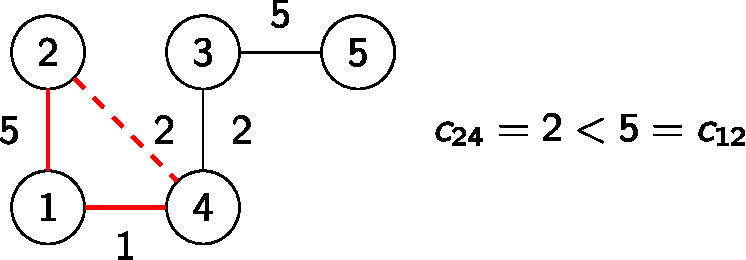
\includegraphics[width=.5\textwidth]{img/trees-opt-condition.pdf}
\end{figure}

\noindent
Because $c\left(T \cup \left\{e\right\} \setminus \left\{f\right\}\right) = c\left(T\right) + c_{e} - c_{f}$, if $e$ is cost decreasing, then:
\begin{equation*}
    c\left(T \cup \left\{e\right\} \setminus \left\{f\right\}\right) < c\left(T\right)
\end{equation*}
\begin{theorem}[Tree optimality condition]
    A tree $T$ is of minimum total cost if and only if no cost-decreasing edge exists.
\end{theorem}
\begin{proof}
    $\Rightarrow$ If a cost-decreasing edge exists, then $T$ is not of minimum total cost.

    $\Leftarrow$ if no cost-decreasing edge exists, then $T$ is of minimum total cost. Let $T^{*}$ be a minimum cost spanning tree found by Prim's algorithm. It can be verified that, by exchanging one edge at a time, $T^{*}$ can be iteratively transformed into $T$ without modifying the total cost. Thus, $T$ is also optimal.
\end{proof}

\noindent
Testing optimality is quite simple. The optimality condition allows to verify whether a spanning tree $T$ is optimal: it suffices to check that each $e \in E \setminus T$ is not a cost-decreasing edge.